\chapter{Теория}
\label{ch:intro}

Ряд Фурье — это способ представить периодическую функцию в виде суммы простых гармонических колебаний 
(синусов и косинусов) с разными частотами, амплитудами и фазами. \\

Функции $\{1, cos(x), sin(x), cos(2x), sin(2x) и т.д\}$ являются базисом пространтсва периодических функций (как в линейной алгебре
есть базис, допустим, трехмерного пространтсва, который состоит из ортов i, j и k, и все вектора в этом пространстве могут быть
разложены по этим ортам, т.е представлены в виде их линеной комбинации), поэтому почти любую периодическую функцию можно представить
в виде суммы функций, принадлежащих этому базису. \\

Еще одним примером разложения является ряд Тейлора. Базисом для пространства функций является множество функций $\{1, x, x^2, x^3, \dots\}$,
по которому также можно разложить почти любую функцию, т.е. представить в виде линейной комбинации многочленов.

Ряд Фурье и его коэффициенты вычисляются следующим образом:

\begin{figure}[H]
    \centering
    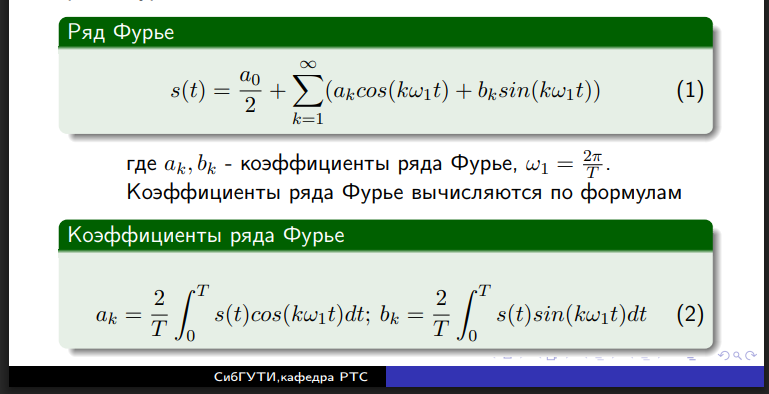
\includegraphics[width=1.0\textwidth]{furie_formula.png}
    \caption{Формула ряда Фурье и коэффициентов}
\end{figure}

где $\frac{a_0}{2}$ "--- постоянная составляющая (или среднее значение сигнала), \\
$a_k$ и $b_k$ "--- коэффициенты ряда Фурье, $a_k$ отвечает за амплитуды чётных (симметричных) составляющих функции
и показывают, насколько сильно в сигнале выражена компонента вида cos($\omega_0t$), а $b_k$ отвечает за амплитуды нечётных (асимметричных) составляющих функции
и показывают, насколько сильно в сигнале выражена компонента вида sin($\omega_0t$). \\
$k$ "--- номер гармоники ($k = 1,2,3,4,\dots$), \\
$\cos(k\omega_1 t)$ и $\sin(k\omega_1 t)$ "--- базисные функции.

Важно заметить, что сигнал, который нужно разложить в ряд Фурье, должен содержать только гармонники с частотой кратной $w_1$. Если
такое условие не выполняется, то сигнал не будет периодическим и разложить его в классический ряд Фурье невозможно.

Пример вычисления коэффициентов ряда Фурье:

\begin{figure}[H]
    \centering
    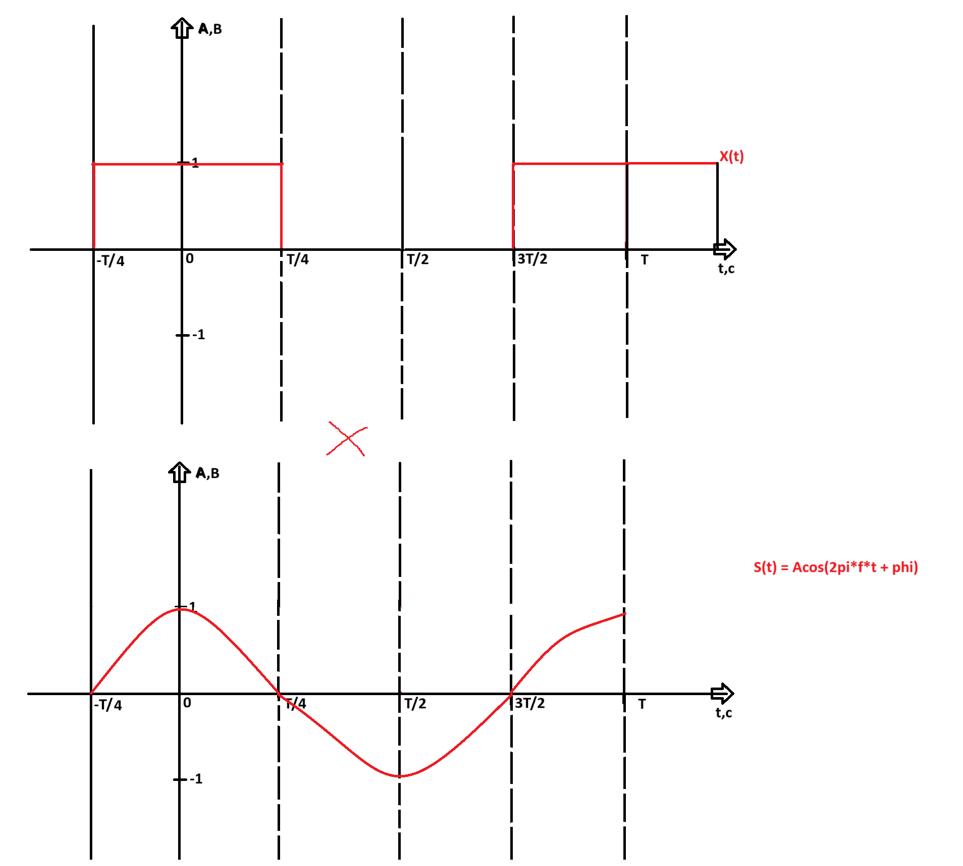
\includegraphics[width=1.0\textwidth]{a_comp_1.png}
    \caption{Геометрическая интерпретация вычисления $a_k$}
\end{figure}


\begin{figure}[H]
    \centering
    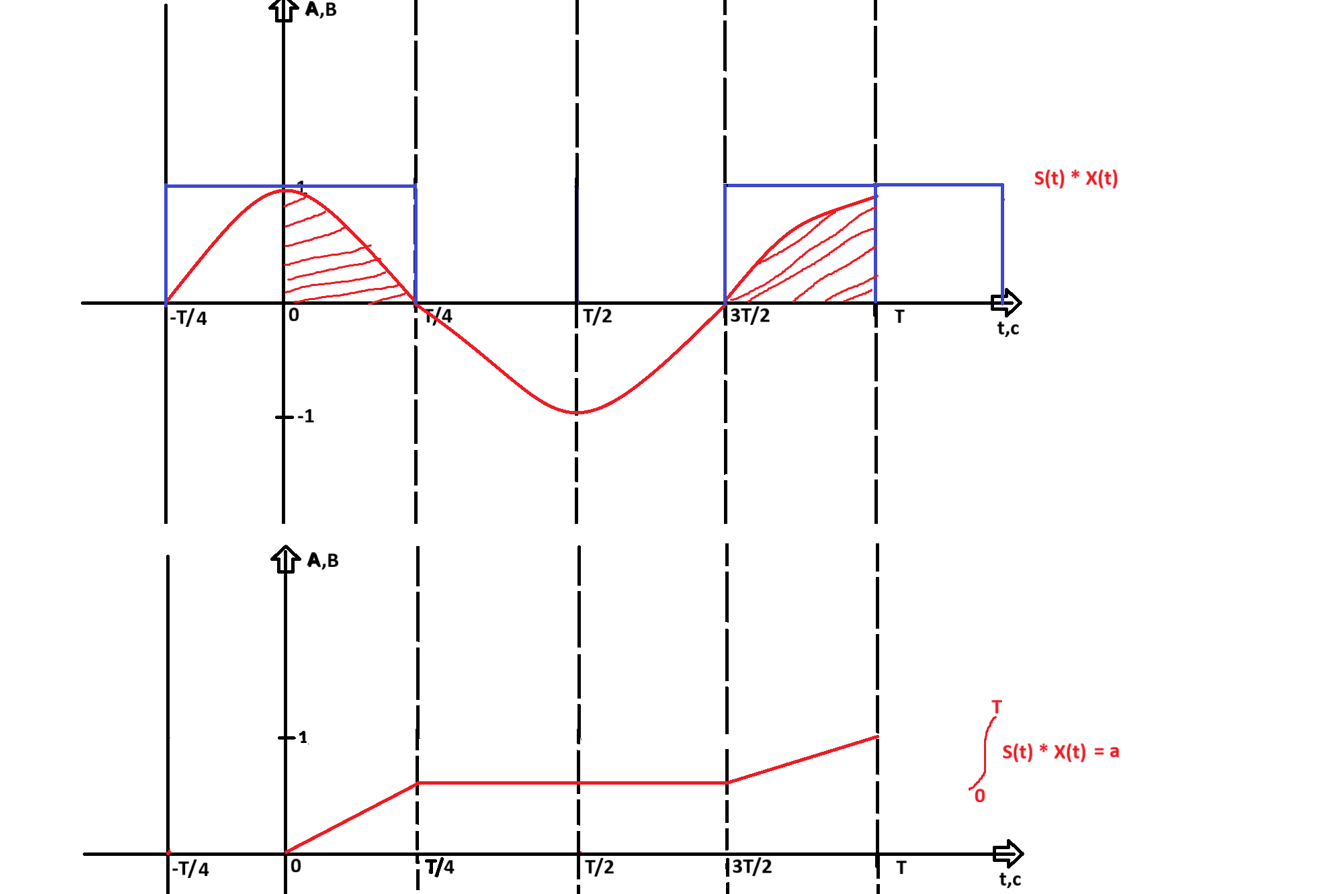
\includegraphics[width=1.0\textwidth]{a_comp_2.png}
    \caption{Геометрическая интерпретация вычисления $a_k$}
\end{figure}

\begin{figure}[H]
    \centering
    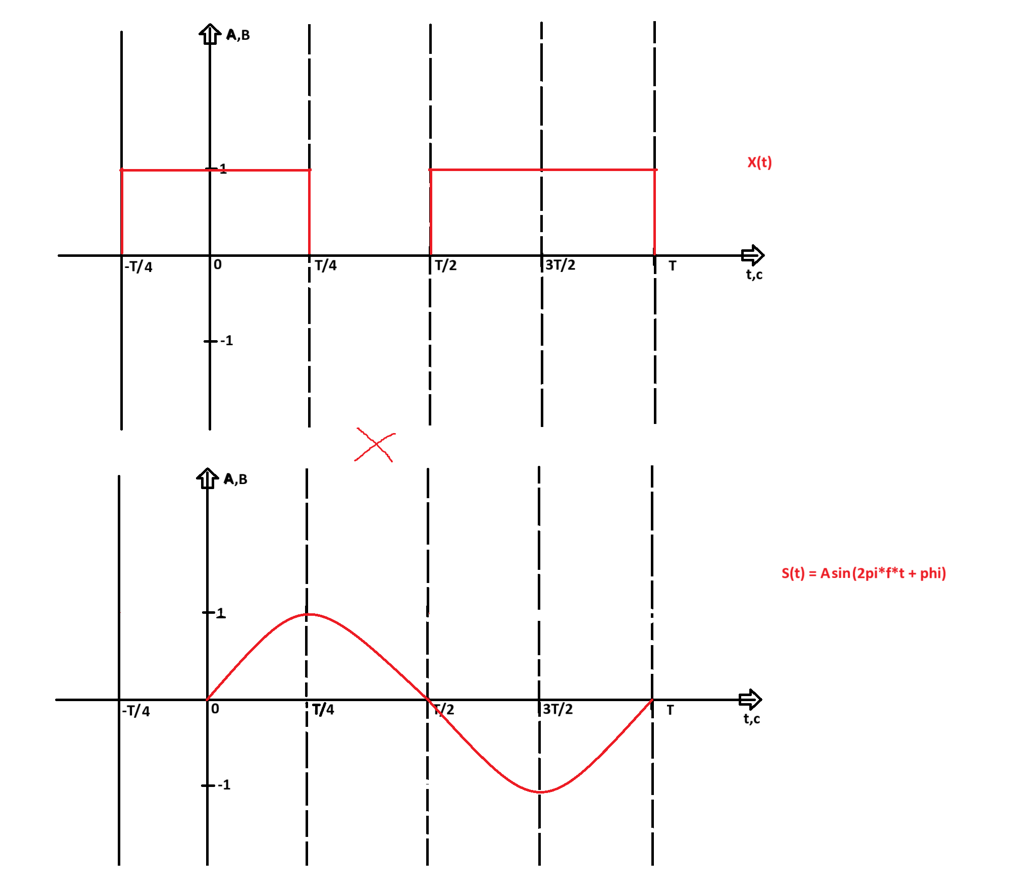
\includegraphics[width=1.0\textwidth]{b_comp_1.png}
    \caption{Геометрическая интерпретация вычисления $b_k$}
\end{figure}


\begin{figure}[H]
    \centering
    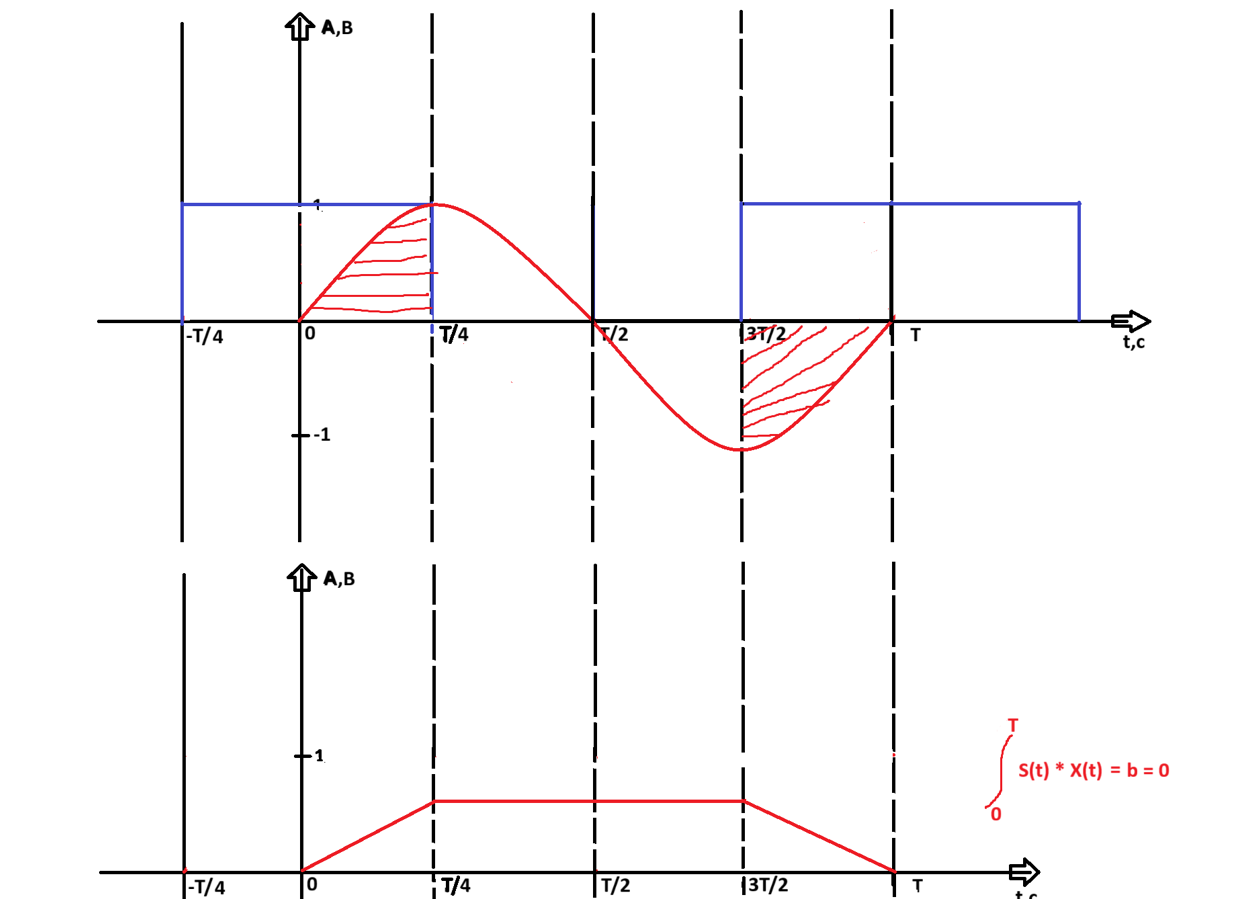
\includegraphics[width=1.0\textwidth]{b_comp_2.png}
    \caption{Геометрическая интерпретация вычисления $b_k$}
\end{figure}

Заметим, что исходный сигнал (прямоугольный) - четный, поэтому коэффциенты $b_k$ будут всегда равны нулю и в разложении
будет участвовать только cos($\omega_0t$).

\subsection*{\textbf{Пример}}

Рассмотрим простейший сигнал $cos(2\pi*t)$. Рассчитаем для него $a_1$ и $b_1$: \\

Перемножим наш сигнал на cos-компоненту при k = 1

\begin{figure}[H]
    \centering
    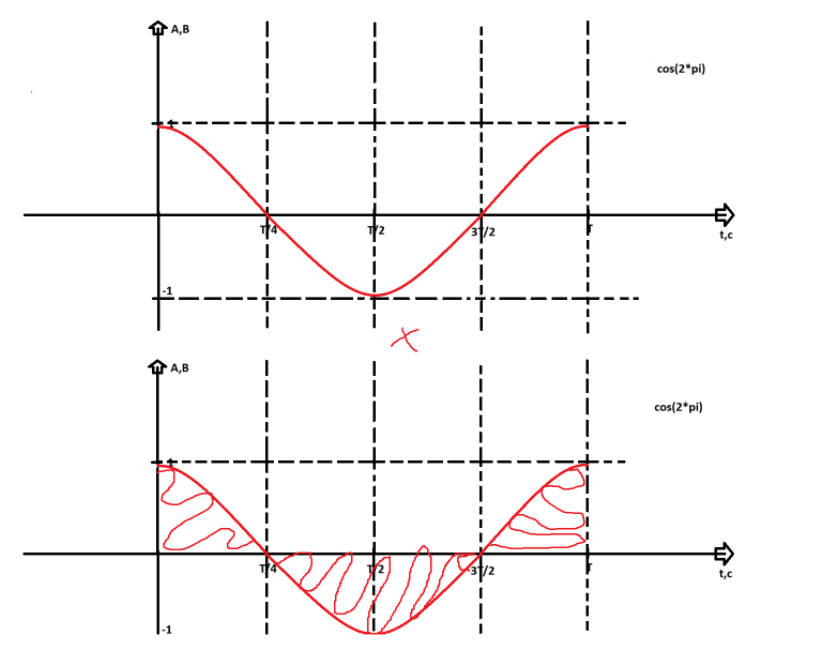
\includegraphics[width=1.0\textwidth]{ex_mul.png}
    \caption{Вычисление $a_1$}
\end{figure}

То, как будет изменяться интеграл от их произведения
\begin{figure}[H]
    \centering
    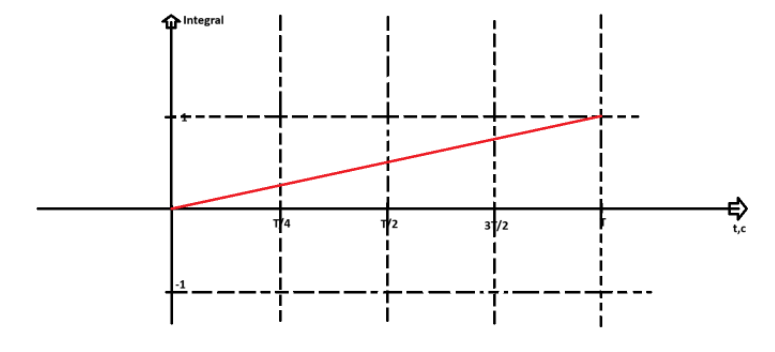
\includegraphics[width=1.0\textwidth]{ex_int1.png}
    \caption{Вычисление $a_1$}
\end{figure}

Значение интеграла в момент времени T будет равно $\pi$, это значит, что в нашем
сигнале присутствует cos-компонента с частотой 1Гц (что логично). \\

Теперь рассчитаем $b_1$, т.е сколько в нашем сигнале содержится компоненты $sin(2\pi*t)$

\begin{figure}[H]
    \centering
    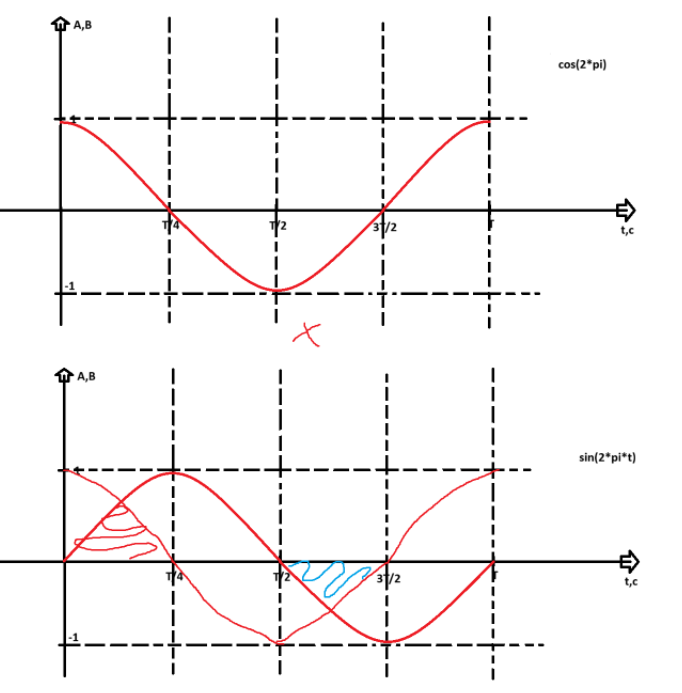
\includegraphics[width=1.0\textwidth]{ex_mul_2.png}
    \caption{Вычисление $a_1$}
\end{figure}

То, как будет изменяться интеграл от их произведения
\begin{figure}[H]
    \centering
    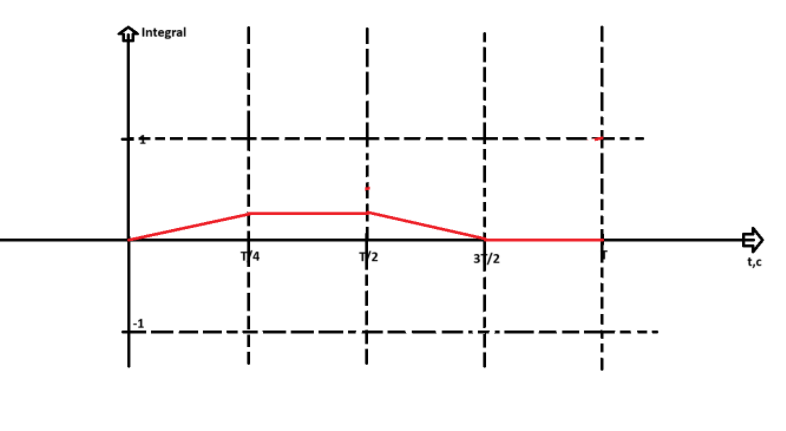
\includegraphics[width=1.0\textwidth]{int2.png}
    \caption{Вычисление $a_1$}
\end{figure}

Значение интеграла в момент времени T будет равно 0, это значит, что в нашем
сигнале не присутствует sin-компонента с частотой 1Гц (что логично, ведь наш сигнал изначально косинус, который симметричен). \\

В нашем сигнале точно нет никаких sin-компонент. Может, есть компонента $cos(4\pi*t)$?


\begin{figure}[H]
    \centering
    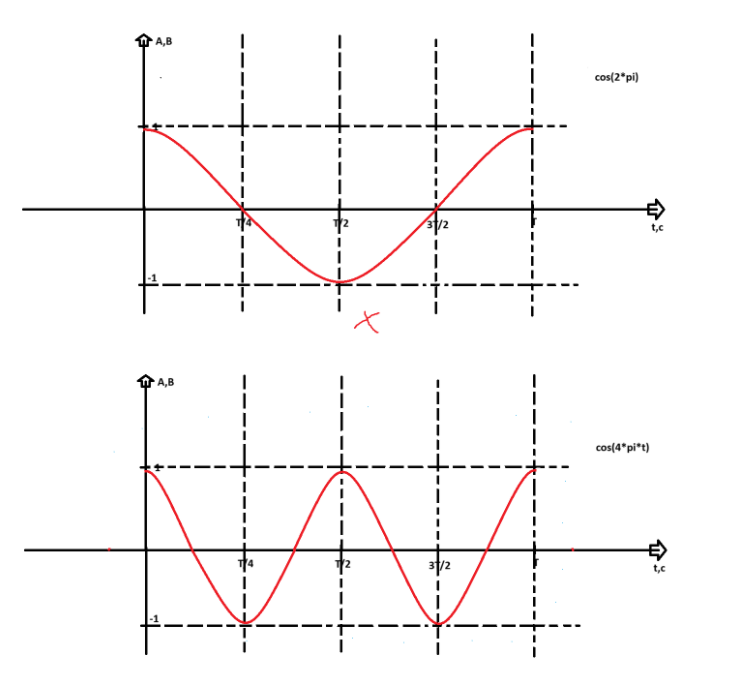
\includegraphics[width=1.0\textwidth]{ex_mul2.png}
    \caption{Вычисление $a_1$}
\end{figure}

То, как будет изменяться интеграл от их произведения
\begin{figure}[H]
    \centering
    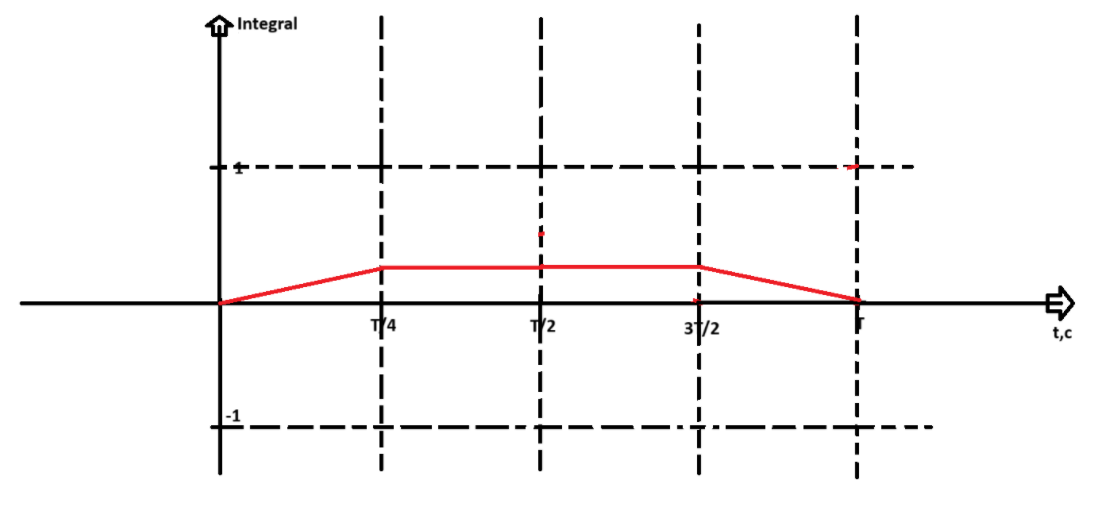
\includegraphics[width=1.0\textwidth]{int3.png}
    \caption{Вычисление $a_1$}
\end{figure}

В графике много симметричностей, которые по итогу дают ноль. При увеличении частоты компонент ничего не поменяется: будут симетричности,
которые в сумме будут сводить интеграл к нулю. Это значит, что в нашем сигнале только 1 компонента $cos(2\pi*t)$. \\

\subsection*{\textbf{Иная форма записи ряда Фурье}}

Классическая форма ряда Фурье не очень удобна для вычисления, поэтому ее заменяют косинусной формой ряда Фурье:

$$\frac{A_0}{2}+\sum_{n=1}^{\inf}A_n*cos(n*\omega_1t+\phi_n)$$

где $A_n = \sqrt{a_n^2+b_n^2}$, а $\phi_n = -arctg(\frac{b_n}{a_n})$

\subsection*{\textbf{Ряд Фуре в комплексной форме}}

Вспомним тригонометрические тождества Эйлера:

\begin{figure}[H]
    \centering
    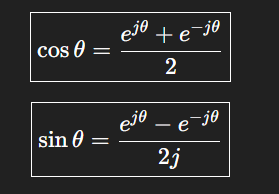
\includegraphics[width=1.0\textwidth]{euler_form.png}
    \caption{Тригонометрические тождества Эйлера}
\end{figure}

Теперь cos в формуле из прошлого пункта заменим соответсвующим тождеством:

\[
\frac{A_0}{2} + \sum_{n=1}^{\infty} A_n \cos\!\bigl(n\omega_1 t + \phi_n\bigr)
= \frac{A_0}{2} + \sum_{n=1}^{\infty} A_n \,\frac{e^{i(n\omega_1 t + \phi_n)} + e^{-i(n\omega_1 t + \phi_n)}}{2}
\]

Видим у экспонент сумму в степени. Преобразуем выражение

\[
\frac{A_0}{2} + \sum_{n=1}^{\infty} A_n \cos\!\bigl(n\omega_1 t + \phi_n\bigr)
= \frac{A_0}{2} + \sum_{n=1}^{\infty} 
\frac{A_n}{2}\left(e^{i\phi_n} e^{i n\omega_1 t} + e^{-i\phi_n} e^{-i n\omega_1 t}\right)
\]

Раскроем скобки:

\[
\frac{A_0}{2} + \sum_{n=1}^{\infty} 
\frac{A_ne^{i\phi_n}}{2} e^{i n\omega_1 t} 
+ \frac{A_ne^{-i\phi_n}}{2} e^{-i n\omega_1 t}
\]

В этой формуле $e^{i n\omega_1 t}$ и $e^{-i n\omega_1 t}$ - колебания. \\

$\frac{A_ne^{i\phi_n}}{2}$ и $\frac{A_ne^{-i\phi_n}}{2}$ - комплексные амплитуды.
Обычно их заменяют на $\dot{C_n}$ и $\dot{C_{-n}}$ соответсвенно. \\

Чтобы не считать 2 коэффициента, можно рассматривать сумму от $-\infty$ до $\infty$ и записать формулу так:

$$\sum_{n=-\infty}^{\infty} C_ne^{in\omega_1t}$$

\textbf{Примечание:} спектр сигнала будет распространяться в отрицательную и положительную сторону. Это не значит, что частота
стала отрицательной, это всего лишь симметрия графика.\\

Вычисление $C_n$:

$C_n = \frac{1}{T}\int_{0}^{T}S(t)*e^{-in\omega_1t}dt$ \\

Установим некоторую взаимосвязь между тригонометрической и комплексной формой ряда Фурье: \\

$A_0 = \dot{C_0}$, что логично, ведь если в формулу для их вычисления подставить 0, то получим одно и то же значение. \\

Теперь обратим внимание, что:

$$\frac{A_n*e^{i\phi_n}}{2} = \dot{C_n} = \lvert\dot{C_n}\rvert * e^{i\phi_n}$$
$$\frac{A_n*e^{-i\phi_n}}{2} = \dot{C_{-n}} = \lvert\dot{C_n}\rvert * e^{-i\phi_n}$$

Из двух уравнений выше следует, что:

$$\lvert\dot{C_n}\rvert = \frac{A_n}{2}$$

Это значит, что коэффициент А тригонометрического ряда Фурье вдвое больше коэффициента $\lvert\dot{C_n}\rvert$ комплексного ряда
Фурье. Это связано с тем, что коэффициентов $\lvert\dot{C_n}\rvert$ вдвое больше (спектр в обе стороны). \\

Коэффициенты ряда Фурье являются комплексно сопряженными, т.е:

$$\dot{C_{-n}} = C_{n}^*$$


\subsection*{\textbf{Прямоугольный сигнал и ряд Фурье для него}}

Прямоугольный сигнал имеет следующие характеристики: \\

$T(s)$ - период (время одного колебания) \\
$\tau(s)$ - длительность сигнала (то время, когда сигнал не равен 0) \\
$U (B)$ - максимальное значение сигнала \\
$q = \frac{T}{\tau}$ - скважность сигнала \\

\begin{figure}[H]
    \centering
    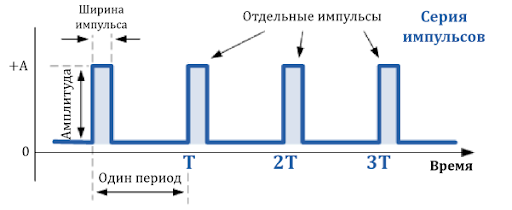
\includegraphics[width=1.0\textwidth]{rect_signal.png}
    \caption{Пример прямоугольного сигнала с обозначением характеристик}
\end{figure}

Для прямоугольного сигнала коэффициент $\dot{C_n}$ вычисляется иначе: интегрирование идет не по T, а по $\tau$

\[
C_n = \frac{1}{T} \int_{-\tau/2}^{\tau/2} U e^{-i n \omega_1 t}\, dt
\]

U не зависит от t, поэтому вынесем ее за интеграл. Вспомним, что $\int e^{ax} = \frac{1}{a}e^x$. Вычислим интеграл:

\[
\frac{U}{T} \cdot \frac{e^{-i n \omega_1 t}}{-i n \omega_1} \Bigg|_{-\tau/2}^{\tau/2}
\]

\[
= \frac{U}{T} \cdot \frac{1}{-i n \omega_1}
\left[
e^{-i n \omega_1 \tfrac{\tau}{2}} - e^{-i n \omega_1 \left(-\tfrac{\tau}{2}\right)}
\right]
\]

\[
= \frac{U}{T} \cdot \frac{1}{-i n \omega_1}
\left[
e^{-i n \omega_1 \tfrac{\tau}{2}} - e^{i n \omega_1 \tfrac{\tau}{2}}
\right]
\]

Теперем заменим $\omega_1$ на $2\pi f_1$ и внесем двойку вместе с i под знак выражения в скобках, n и $\pi f_1$ занесем в первый множитель:

\[
\frac{U}{Tn\pi f_1} \cdot \frac{e^{i n \omega_1 \tfrac{\tau}{2}} - e^{-i n \omega_1 \tfrac{\tau}{2}}}{2i}
\]

Видим $sin(n\omega_1\frac{\tau}{2})$ (по тригонометрическому тождеству Эйлера):

\[
\frac{U}{Tn \pi f_1} \cdot \sin\!\left(n \omega_1 \frac{\tau}{2}\right)
\]

Заменим $\omega_1$ под синусом на $2\pi f_1$ и $f_1$ запишем как $\frac{1}{T}$. $n \pi f_1$ из знаменателя первого множителя внесем в знаменатель второго:

\[
\frac{U}{T} \cdot \frac{\sin\!\left(n \pi \frac{\tau}{T}\right)}{n \pi \frac{1}{T}}
\]

Теперь домножим числитель и знаменатель на $\tau$

\[
\frac{U \tau}{T} \cdot \frac{\sin\!\left(n \pi \frac{\tau}{T}\right)}{n \pi \frac{\tau}{T}}
\]

Все эти преобразования нужны были для того, чтобы торой множитель превратился в один из замечательных пределов, который  на бесконечности стремится к единице. \\

Итоговая формула для вычисления коэффициентов в комплексной форме ряда Фурье для прямоугольного периодического сигнала:

\[
\boxed{\frac{U \tau}{T} \cdot \frac{\sin\!\left(n \pi \frac{\tau}{T}\right)}{n \pi \frac{\tau}{T}}}
\]

\subsection*{\textbf{Ортогональность сигнала}}

Два сигнала \(x(t)\) и \(y(t)\) называются \textbf{ортогональными} на интервале \([a, b]\), если их скалярное произведение равно нулю:

\[
\langle x, y \rangle = \int_{a}^{b} x(t) \, y(t) \, dt = 0
\]

Это означает, что сигналы в радиоканале "не мешают" друг другу, т.е не заглушают друг друга их их можно передавать вместе. Эта идея используется в таких
технологиях, как CDMA и OFDM.
\endinput